\section{Motivation} \label{sec:motivation}
By relaxing the design constraints, we can take advantage of the neural network 
fault-tolerance and obtain significant improvements on 
performance or energy efficiency with moderate computing errors but small prediction 
accuracy loss. While the neural network model resilience is key to the  
design trade-offs, we take overclocking as an example of accelerators 
with computing errors, analyze the influence of computing errors on 
the neural network model prediction accuracy. The widely used neural 
training techniques such as training with noisy data and dropout may be 
utilized to improve neural network model resilience and they are also 
evaluated.

We used PipeCNN\cite{pipecnn_2}, an open sourced high-level CNN accelerator, 
as the baseline design. We had it implemented on KCU1500 FPGA board. 
On ImageNet, we trained AlexNet, VGG16 and VGG19 offline and then applied 
them to the 8bit CNN accelerator. When the accelerator is overclocked and 
the clock is boosted to the extreme case where 
further overclocking will lead to frequent hardware crash, we measure the prediction accuracy of 
the three typical neural networks and compare with that obtained from accelerators with normal 
clocking. In addition, we also evaluate the models trained with noisy data and dropout and 
compare with the original model.

Figure \ref{fig:top1-loss} and Figure \ref{fig:top5-loss} show the top1 and top5 prediction accuracy comparison 
respectively. It can be found that all the three neural network models suffer considerable accuracy loss 
when the models are deployed on the overclocked accelerator directly. The average top1 accuracy and top5 accuracy 
drops by 17.1\% and 29.8\% respectively, which undermines the usefulness of overclocking dramatically.
Particularly, top1 accuracy drops more than top5 accuracy on all the 
models, which means that the top1 of the final softmax output changes but it probably 
stays in the top5 range. 

We also evaluated the models trained with noisy data and dropout. 
The comparison reveals that offline training with dropout can hardly 
improve the resilience of the neural network models and even lowers the 
prediction accuracy slightly when the models are executed on the 
overclocked accelerator. While neural network models trained with 
noisy data have distinct influence on different models, the 
prediction accuracy of AlexNet drops but the accuracy of VGG16 
improves. The prediction accuracy of VGG19 does not change much.
It indicates that computing errors caused by the noisy data are 
different from that incurred by overclocking. The difference varies 
in different neural network models and there is no guarantee 
for the accuracy improvement using noisy data training.
\begin{figure}
        \center
        \subfloat[top1 prediction accuracy]{
                \label{fig:top1-loss}
                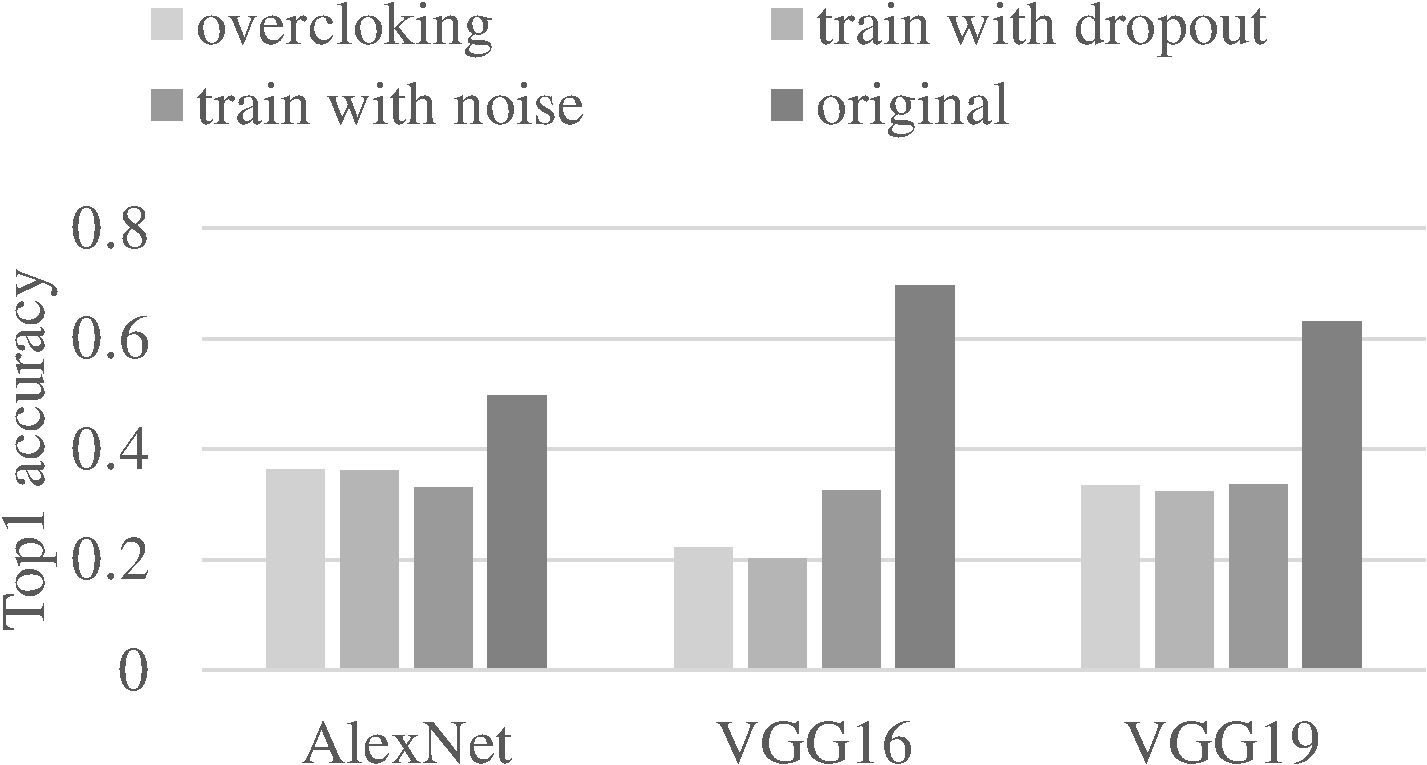
\includegraphics[width=0.7\linewidth]{top1_dropout_noisy}
        }
        \qquad
        \subfloat[top5 prediction accuracy]{
                \label{fig:top5-loss}
                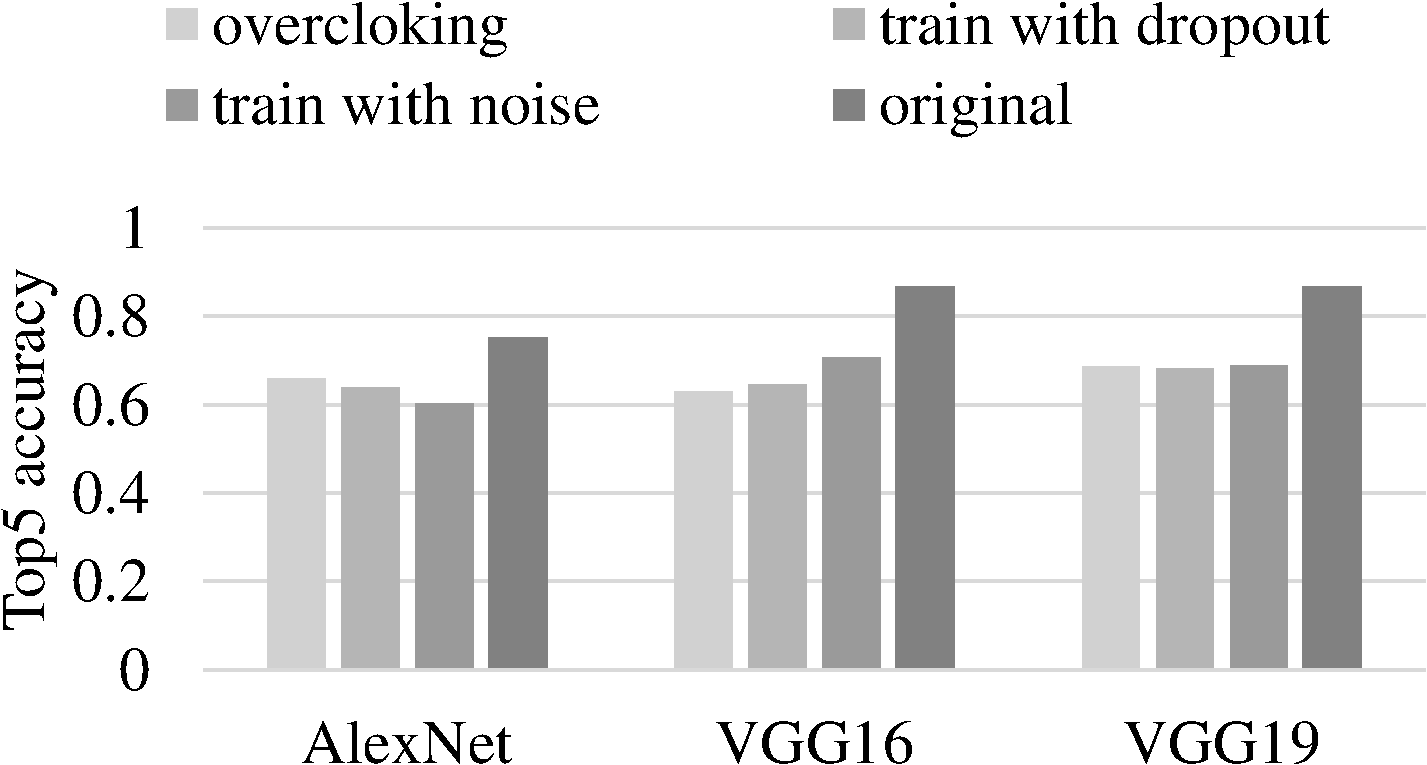
\includegraphics[width=0.7\linewidth]{top5_dropout_noisy}
        }
        \caption{Prediction accuracy loss of models running on overclocked CNN accelerators.
			'Overclocking' refers to the neural networks models running on overclocked accelerators. 
'train with dropout' and 'train with noise' represent the models trained with dropout strategy 
and noisy data respectively. They are also applied on overclocked accelerators. 
'Original' means the models running on normal accelerator.
 }
 \vspace{-1em}
        \label{fig:accuracy-dropout-noisy}
\end{figure}

To gain further insight of the computing errors, we analyze the error distribution 
of different layers when compared to the correct execution. Based on the error range, 
we divide the errors into 3 categories including R0 ($error = 0$), 
R1 ($0 \leq error \leq 5$) and R2 ($error > 5$). As shown in 
Figure \ref{fig:error_distribute}, most of the computing results remain 
correct even in the extreme overclocking scenario. Full connection (FC) in the last layer 
has only a small portion of correct computing results and most of the computing errors are 
larger than 5. As the last layer is close to the result and affects the final output 
directly, it becomes a critical layer that limits the overall resilience of the neural 
networks. 

\begin{figure*}
        \center{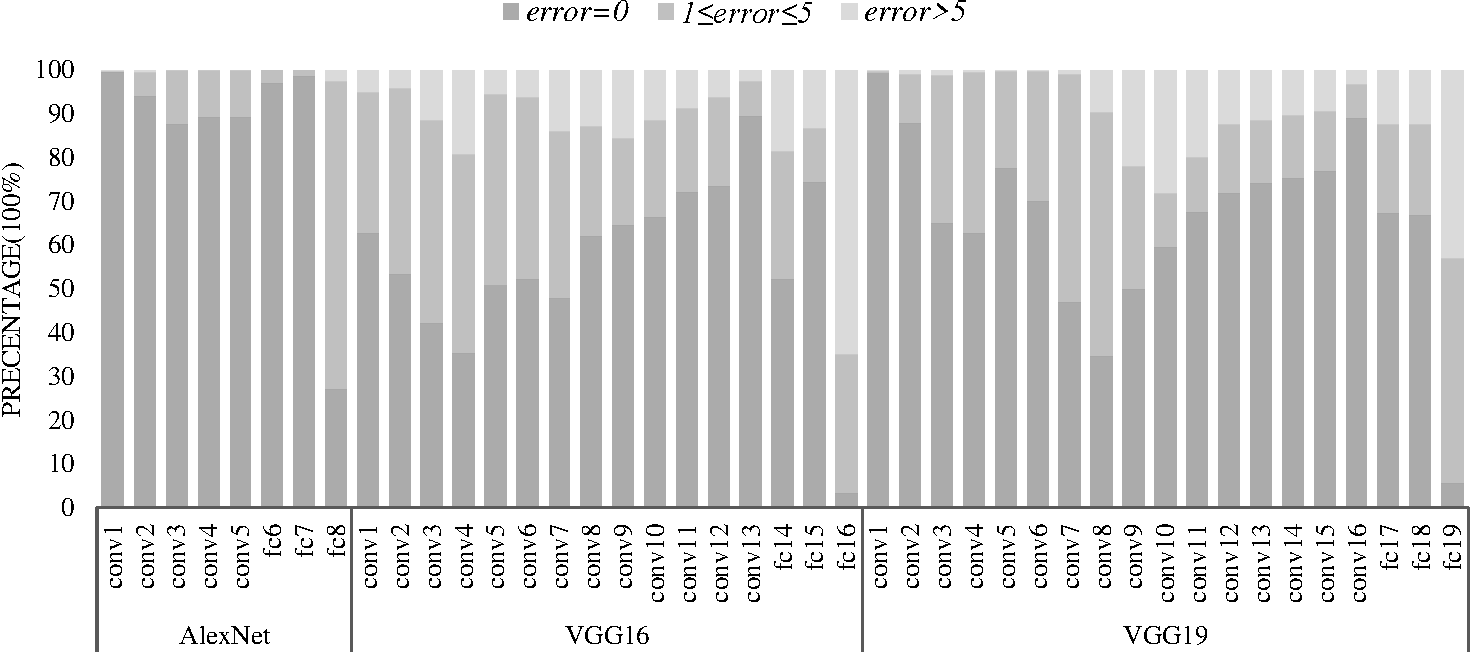
\includegraphics[width=0.8\linewidth]{error_distribute}}
        \caption{Computing error distribution across the different layers when executed on overclocked CNN accelerator}
        \label{fig:error_distribute}
\end{figure*}

According to the experiments, we observe that the computing errors induced by 
overclocking can lead to dramatic prediction accuracy loss, though 
the neural networks are usually resilient. The errors are rather difficult to be
covered via offline training with noisy data and dropout. 
Instead of training on GPPs, we try to integrate the accelerator in the training framework 
such that computing errors can be considered during training directly. In addition, we notice 
that the last layer typically suffer more large errors, so we opt to protect the last layer 
that takes up only a small portion of the neural network computing. By scheduling it to GPPs 
or other infrastructures without errors may improve the resilience of the overall neural 
networks, which allows more advantageous design trade-offs.

